\documentclass{article}
\usepackage{v-test-paper}
\title{\textsc{Circular Motion}}
\date{February 24, 2024}

\newcommand{\itemstared}{\refstepcounter{enumi}\item[$^\star$\theenumi.]}
\usetikzlibrary{matrix,  positioning, patterns, backgrounds}
\renewcommand{\ans}{\quad}


\tikzstyle{root} = [rectangle, rounded corners, 
minimum width=3cm, 
minimum height=0.7cm,
text centered, 
draw, 
font=\scshape,
]
\tikzstyle{child} = [rectangle, rounded corners, 
inner sep=2mm,
text centered, 
draw, 
font=\itshape,
text width=3.25cm,
]

\tikzstyle{child-branch} = [
    rectangle, 
    rounded corners, 
    inner sep=2mm,
    text centered, 
    draw, 
    font=\itshape,
    text width=2.5cm,
    level distance=5mm,
]



\tikzstyle{arrow} = [thick,->,>=latex]


\begin{document}
\maketitle
\begin{center}
\begin{tikzpicture}[node distance=2cm]

\matrix [column sep=5mm,row sep=10mm]
{
&\node (root) [root] {Circular Motion};\\
\node (child-left)[child] {Kinematics}; & &
\node (child-right)[child] {Dynamics}; \\
\node (child-left-b)[child] {Angular Velocity, Linear Velocity}; & &
\node[child-branch](child-right-bl)at ($(child-right.south)+(-1.5, 0)$){Centripetal Force}; 
\node[child-branch](child-right-br)at ($(child-right.south)+(1.5, 0)$){Centrifugal Force}; \\
\node (child-left-bb)[child] {Acceleration}; & &
\node[child-branch](child-right-blb)at ($(child-right-bl.south)+(0, 0)$){Conical Pendulum, Rotor, Circular track(Banking + Friction)}; 
\node[child-branch](child-right-brb)at ($(child-right-br.south)+(0, 0)$){Motion in a vertical circle};\\
\node[child-branch](child-left-bbl)at ($(child-left.south)+(-1.5, 0)$){Uniform Circular Motion, Only radial acceleration}; 
\node[child-branch](child-left-bbr)at ($(child-left.south)+(1.5, 0)$){Non-Uniform Circular Motion, Radial + tangential acceleration}; & &\\
};

\draw [arrow] (root) -| (child-left);
\draw [arrow] (root) -| (child-right);
\draw [arrow] (child-left) --(child-left-b);
\draw [arrow] (child-right) -- (child-right-bl);
\draw [arrow] (child-right) -- (child-right-br);
\draw [arrow] (child-left-bb)--(child-left-bbl);
\draw [arrow] (child-left-bb)--(child-left-bbr);
\draw [arrow] (child-left-b)--(child-left-bb);
\draw [arrow] (child-right-bl)--(child-right-blb);
\draw [arrow] (child-right-br)--(child-right-brb);
\end{tikzpicture}
\end{center}

\begin{center}
    \textsc{Problems}
\end{center}
\begin{enumerate}
    \item A particle is moving in a circle of radius $R$ in such a way that at any instant the normal and tangential component of its acceleration are equal. If its speed at $t = 0$ is $v_0$. The time taken to complete the first revolution is
        \begin{tasks}(2)
            \task $\dfrac{R}{v_0}$
            \task $\dfrac{R}{v_0}e^{-2\pi}$
            \task $\dfrac{R}{v_0}\left(1-e^{-2\pi}\right)$\ans
            \task $\dfrac{R}{v_0}\left(1+e^{-2\pi}\right)$
        \end{tasks}

    \item A particle is describing circular motion in a horizontal plane in contact with the smooth surface of a fixed right circular cone with its axis vertical and vertex down. The height of the plane of motion above the vertex is $h$ and the semi-vertical angle of the cone is $\alpha$. The period of revolution of the particle
    \begin{center}
        \begin{tikzpicture}
            \def\angle{60}
            \tzcoor(0, 0)(O)
            \tzcoor(\angle:3)(A)
            \tzcoor(180-\angle:3)(B)
            \tzcoor*(2*cos{\angle}, 2*sin{\angle})(C)(4pt)
            \tzcoor(3, 0)(C)
            \tzline(O)(A)
            \tzline(O)(B)
            \tzline(O)(C)
            \tzanglemark(C)(O)(A){$\alpha$}
            \tzellipse[dashed](0, 2*sin{\angle})(2*cos{\angle} and 0.3)
            \tzline+[|<->|]<1.5, 0>(0, 0)(0, 2*sin{\angle}){$h$}[mr]
        \end{tikzpicture}
    \end{center}
    \begin{tasks}(2)
        \task increases as $h$ increases\ans
        \task decreases as $h$ decreases
        \task increases as $\alpha$ increases
        \task decreases as $\alpha$ increases\ans
    \end{tasks}

    \item The speed of a particle moving in a circle of radius $r = 2 \m$ varies with time $t$ as $v = t^2$, where $t$ is in second and $v$ in $\mps$. Find the net acceleration at $t = 2 \s$.
    \begin{tasks}(2)
        \task $\sqrt{80}\mpss$\ans
        \task $4\mpss$
        \task $8\mpss$
        \task $\sqrt{8}\mpss$
    \end{tasks}

    \item A table with smooth horizontal surface is turning at an angular speed $\omega$ about its axis. A groove is made on the surface along a radius and a particle is gently placed inside the groove at a distance $a$ from the center. Find the speed of the particle as its distance from the center becomes $L$.
    \begin{center}
        \begin{tikzpicture}
            \tzcoor*(0, 0)(O)
            \tzcoor*(1.5, 0)(A)(3.5pt)
            \tzellipse(O)(3 and 1)
            \tzline[dashed](0, -2)(0, 2)
            \tzarc[->](0, 1.8)(-100:150:0.25 and 0.1){$\omega$}[l]
            \tzrectangle[rounded corners](0, -0.08)(3, 0.08)
            \tzline[|<->|]<0, 0.25>(O)(A){$a$}[ma]
            \tzline+[->]<0, -0.25>(A)(1, 0){$v$}[r]
        \end{tikzpicture}
    \end{center}
    \begin{tasks}(2)
        \task $2\omega\sqrt{L^2-a^2}$
        \task $\omega\sqrt{L^2-a^2}$\ans
        \task $\omega\sqrt{L^2+a^2}$
        \task $2\omega\sqrt{L^2+a^2}$
    \end{tasks}

    \item A turn of radius $20\m$ is banked for the vehicle of mass $200\kg$ going at a speed of $10\mps$. Find the direction and magnitude of the frictional force acting on the vehicle if it moves with a speed of $15\mps$.
    \begin{tasks}(2)
        \task $500\sqrt{5}\N$ up the incline
        \task $500\sqrt{5}\N$ down the incline \ans
        \task $300\sqrt{5}\N$ up the incline
        \task $300\sqrt{5}\N$ down the incline
    \end{tasks} 

    \item With what minimum speed $v$ must a small ball should be pushed inside a smooth vertical tube from a height $h$ so that it may reach the top of the tube? Radius of the tube is $R$. Inner diameter of the tube is $d\ll R$.
        \begin{center}
            \begin{tikzpicture}
                \tzcoor*(0, 0)(O)
                \def\R{2.5}
                \def\r{2}
                \tzcircle(O)(\r)
                \tzcircle(O)(\R)
                \tzdot*(-150:0.5*\R + 0.5*\r)(12pt)
                \tzline[->](O)(60:\r){$R$}[ml]
                \tzline[->](\r-0.5, 0)(\r, 0)
                \tzline[->](\R+0.5, 0)(\R, 0){$d$}[br]
                \tznode(1.5*\R, 0){$d\ll R$}
                \tzline[|<->|]<-\R, 0>(0, -\R)(0, -\R + cos{60}*\R){$h$}[ml]
                \tzline+[->](-150:0.5*\R + 0.5*\r)(-45:0.75){$v$}[br]
            \end{tikzpicture}
        \end{center}
        \begin{tasks}(2)
            \task $\sqrt{2g\left(2R-h\right)}$\ans
            \task $\sqrt{2g\left(2R+h\right)}$
            \task $\sqrt{2g\left(R-h\right)}$
            \task $\sqrt{2g\left(R+h\right)}$
        \end{tasks}

    \item A skier plans to ski a smooth fixed hemisphere of radius $R$. He starts from rest from a curved smooth surface of height $\dfrac{R}{4}$. The angle $\theta$ at which he leaves the hemisphere is
    \begin{center}
        \begin{tikzpicture}
            \tzcoor*(0, 0)(O){$O$}[b]
            \tzarc(0, 0)(0:180:2)
            \tzline[->](O)(45:2){$R$}[mb]
            \tzline[dashed](O)(0, 2)
            \tzanglemark(45:2)(O)(0, 2){$\theta$}(12pt)
            \tzline[dashed](-2, 0)(2, 0)
            \tzline[dashed](-3, 2)(0, 2)
            \tzto[out=-90, in=180](-2.5, 3.5)(0, 2)
            \tzline+[|<->|]<-2.5, 0>(0, 2)(0, 1.5){$\dfrac{R}{4}$}[ml]
        \end{tikzpicture}
    \end{center}
    \begin{tasks}(2)
        \task $\cos^{-1}\left(\dfrac{2}{3}\right)$
        \task $\cos^{-1}\left(\dfrac{5}{\sqrt{3}}\right)$
        \task $\cos^{-1}\left(\dfrac{5}{6}\right)$\ans
        \task $\cos^{-1}\left(\dfrac{5}{2\sqrt{3}}\right)$
    \end{tasks}

    \item Figure shows the total acceleration and velocity of a particle moving clockwise in a circle of radius $R=2.5\m$ at a given instant of time. For this given instant, select the correct option/options.
    \begin{center}
        \begin{tikzpicture}
            \tzcoor*(0, 0)(O)
            \def\R{2}
            \tzcircle(O)(\R)
            \tzline[->](O)(120:\R){$2.5\m$}[ml]
            \tzline(O)(60:\R)
            \tzdot*(60:\R)(4pt)
            \tzline+[->]($(O)+(60:\R)$)(-90:\R){$a=25\mpss$}[b]
            \tzline+[->]($(O)+(60:\R)$)(-30:\R){$v$}[r]
            \tzanglemark(O)(60:\R)(-60:\R){$30^\circ$}(20pt)
        \end{tikzpicture}
    \end{center}
    \begin{tasks}(2)
        \task $v=7.35\mps$\ans
        \task $a_t=12.5\mpss$\ans
        \task $a_r=21.65$\ans
        \task $v=5.59\mps$
    \end{tasks}

    

    
    \begin{center}
        \textsc{Comprehension Based Questions}
    \end{center}
    A small particle of mass $m$ attached with a light inextensible thread of length $L$ is moving in a vertical circle. In the given case particle is moving in complete vertical circle and ratio of its maximum to minimum velocity is $2 : 1$.
    \begin{center}
        \begin{tikzpicture}
            \tzcoor*(0, 0)(O){$O$}[al]
            \tzcoor*(0, -2)(B){$m$}[bl](5pt)
            \tzcircle[dashed](O)(2)
            \tzline(O)(B){$L$}[mr]
        \end{tikzpicture}
    \end{center}
    \item Minimum velocity of the particle is
    \begin{tasks}(2)
        \task $4\sqrt{\dfrac{gL}{3}}$
        \task $2\sqrt{\dfrac{gL}{3}}$\ans
        \task $\sqrt{\dfrac{gL}{3}}$
        \task $3\sqrt{\dfrac{gL}{3}}$
    \end{tasks}

    \item Kinetic energy of the particle at the topmost point is
    \begin{tasks}(2)
        \task $\dfrac{4mgL}{3}$
        \task $\dfrac{8mgL}{3}$\ans
        \task $\dfrac{2mgL}{3}$
        \task $2mgL$
    \end{tasks}

    \item Velocity of the particle when it is moving vertically downward is
    \begin{tasks}(2)
        \task $\sqrt{\dfrac{10gL}{3}}$\ans
        \task $2\sqrt{\dfrac{gL}{3}}$
        \task $\sqrt{\dfrac{8gL}{3}}$
        \task $\sqrt{\dfrac{13gL}{3}}$
    \end{tasks}
    \pagebreak

    \item Speed of a particle moving in a circle of radius $2 \m$ varies with time as $v = 2t$ (SI units). At $t = 1 \s$ match the following two columns :
    \begin{center}
        \renewcommand{\arraystretch}{1.5}
        \begin{table}[h]
            \centering
            \begin{tabular}{p{4cm}|p{3cm}}
            \hline
            Column I & Column II \\
            \hline
            (a) $\vec{a}\cdot \vec{v}$ & (p) $2\sqrt{2}$\\
            (b) $|\vec{a}\times \vec{\omega}|$ & (q) $2$\\
            (c) $\vec{v}\cdot\vec{\omega}$ & (r) $4$\\
            (d) $|\vec{v}\times \vec{a}|$ & (s) None\\
            \hline
            \end{tabular}
        \end{table}
    \end{center}
    \begin{tasks}(2)
        \task $a \rightarrow p, b \rightarrow s, c \rightarrow r, d \rightarrow p$
        \task $a \rightarrow q, b \rightarrow r, c \rightarrow s, d \rightarrow p$
        \task $a \rightarrow r, b \rightarrow p, c \rightarrow s, d \rightarrow r$\ans
        \task $a \rightarrow s, b \rightarrow p, c \rightarrow q, d \rightarrow r$
    \end{tasks}

    \item A bob of mass $m$ is suspended from point $O$ by a massless string of length $l$ as shown. At the bottom-most point it is given a velocity $u = \sqrt{12gl}$ for $l = 1 \m$ and $m = 1 \kg$, match the following two columns when string becomes horizontal ($g = 10 \mpss$ )
    \begin{center}
        
\begin{tikzpicture}
            \tzcoor*(0, 0)(O){$O$}[al]
            \tzcoor*(0, -3)(B){$B$}[bl](5pt)
            \tzline+(O)(B){$l$}[mr]
            \tzline+[->](B)(1, 0){$u$}[r]
        \end{tikzpicture}
    \end{center}
    \begin{center}
        \renewcommand{\arraystretch}{1.5}
        \begin{table}[h]
            \centering
            \begin{tabular}{p{6cm}|p{3cm}}
            \hline
            Column I & Column II \\
            \hline
            (a) Speed of bob & (p) $10$\\
            (b) Acceleration of bob & (q) $20$\\
            (c) Tension in string & (r) $100$\\
            (d) Tangential acceleration of bob & (s) None\\
            \hline
            \end{tabular}
        \end{table}
    \end{center}
    

    \begin{tasks}(2)
        \task $a \rightarrow p, b \rightarrow s, c \rightarrow r, d \rightarrow p$\ans
        \task $a \rightarrow q, b \rightarrow r, c \rightarrow s, d \rightarrow p$
        \task $a \rightarrow r, b \rightarrow p, c \rightarrow s, d \rightarrow r$
        \task $a \rightarrow s, b \rightarrow p, c \rightarrow q, d \rightarrow r$
    \end{tasks}



\end{enumerate}


% \pagebreak
\vspace*{\fill}

\begin{center}
\texttt{Answer Key}
\begin{multicols}{5}
\begin{enumerate}
\item (b)
\item (a)
\item (b)
\item (c)
\item (d)
\item (a)
\item (b)
\item (c)
\item (a)
\item (a)
\item (b)
\item (a)
\item (b)
\item (a)
\end{enumerate}
\end{multicols}
\end{center}






\end{document}